\section{Simulation of the modified controller}
Now we will simulate our system with the same initial conditions as previously and the modified control law given in section 4. Let $k_p = 10$ and $k_d = 300.$
The desired quaternion $\mathbf{q_d}$  is the one corresponding to the following Euler angles: 
\begin{align*}
    \phi(t) &= 10 \sin{0.1t} \\
    \theta(t) &= 0 \\
    \psi(t) &= 15 \cos{0.05t}
\end{align*}

See figure \ref{fig:eulang2}, \ref{fig:eulang_tilde2} and \ref{fig:tau2}  for the plots of the Euler angles (both actual and desired) and angular velocities ($\phi, \phi_d, \theta, \theta_d, \psi, \psi_d, \boldsymbol{\omega}$), the Euler angles error ($\tilde \phi, \tilde \theta, \tilde \psi$) and the control inputs ($\boldsymbol{\tau}$).

The behavior of the system does not match our expectations as the angles $\phi$ and $\psi$ do not follow their desired sinusoidal states. The angle $\theta$ reaches its desired state of 0 degrees, but slower than in the previous simulation. These errors are caused by the fact that the desired states of $\omega_1$, $\omega_2$ and $\omega_3$ are set to 0, while the desired states of $\mathbf{q}$ are set to follow trigonometric functions. This results in opposing forces, some that try to follow sinusoidal signals, and others that try to keep the satellite still.\\
As we can see from the graphs, the Euler angles are both trying to approach zero (because of $\mathbf{\omega_d}$) and oscillate at the same time (due to $\mathbf{q_d}$).


\begin{figure}[h!]
    \centering
    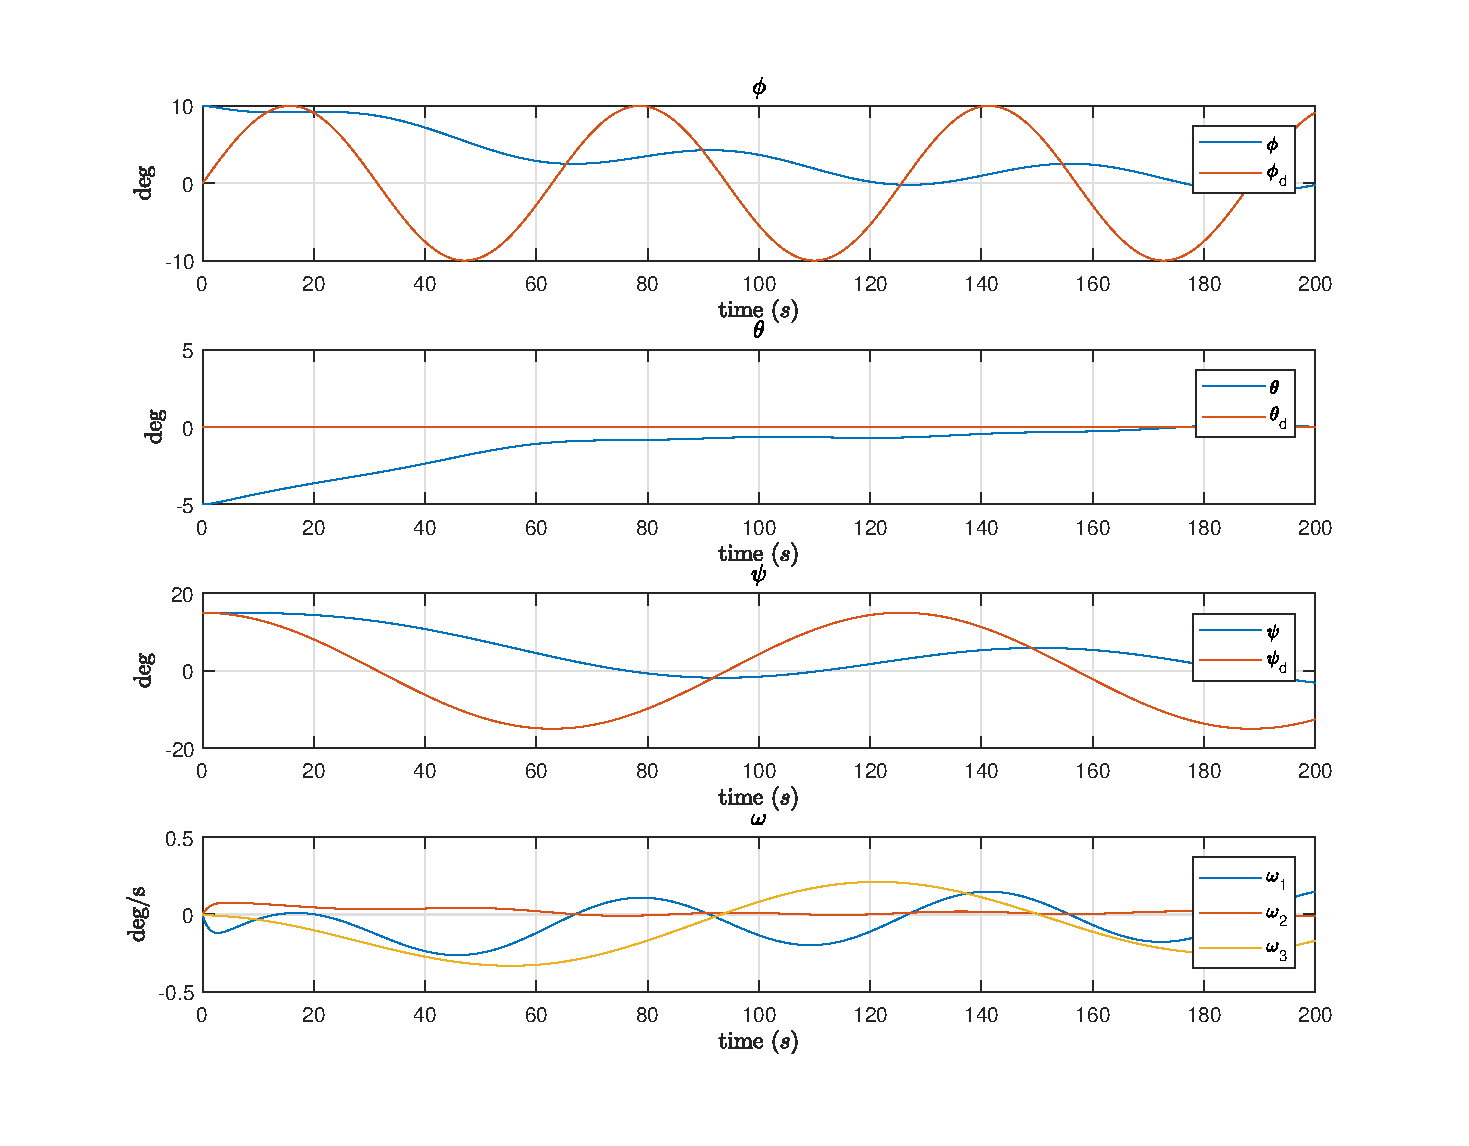
\includegraphics[scale=0.65]{eulang2.eps}
    \caption{Simulated euler angles and angular velocity}
    \label{fig:eulang2}
\end{figure}

\begin{figure}[h!]
    \centering
    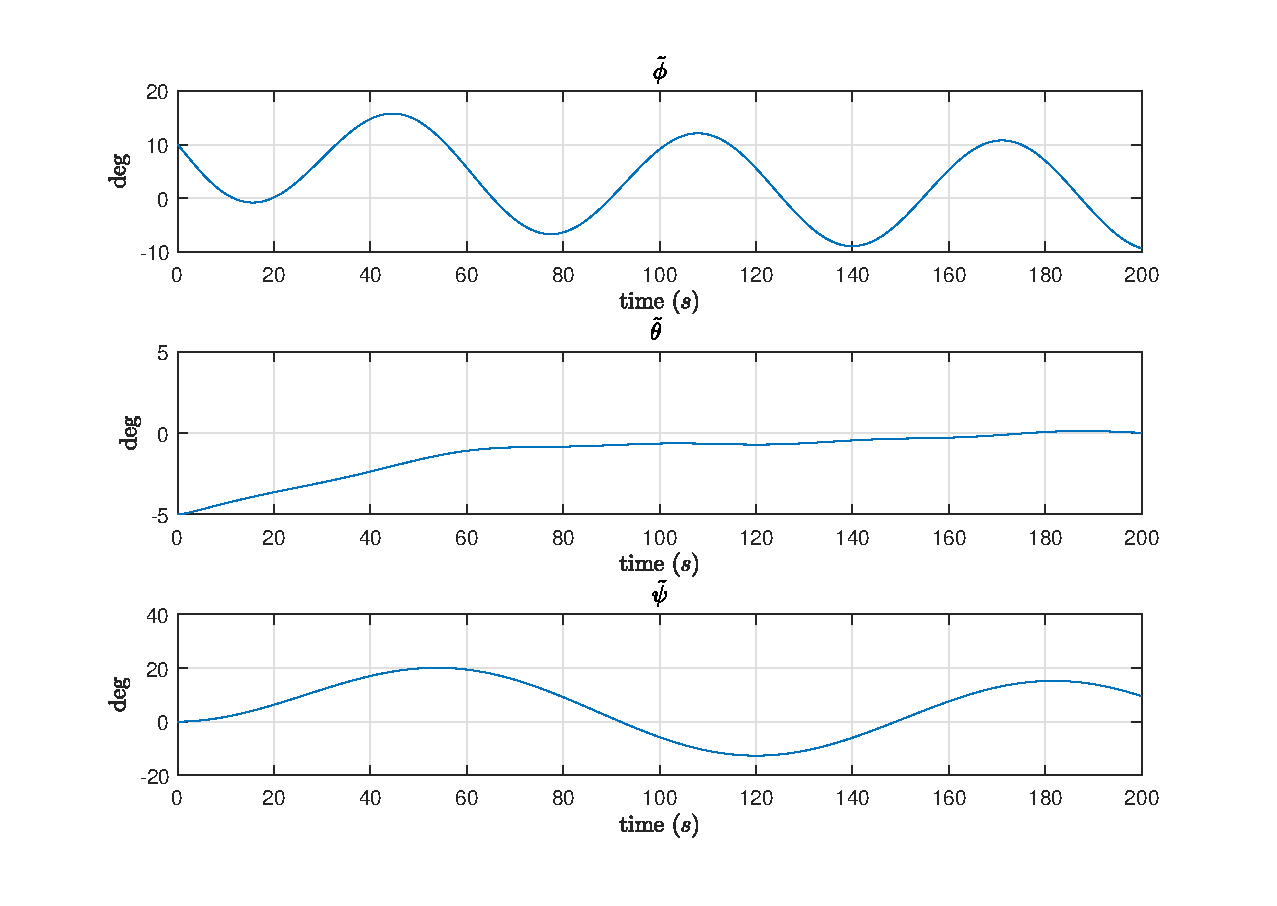
\includegraphics[scale=0.7]{eulang_tilde2.eps}
    \caption{Simulated Euler angles tracking error}
    \label{fig:eulang_tilde2}
\end{figure}

\begin{figure}[h!]
    \centering
    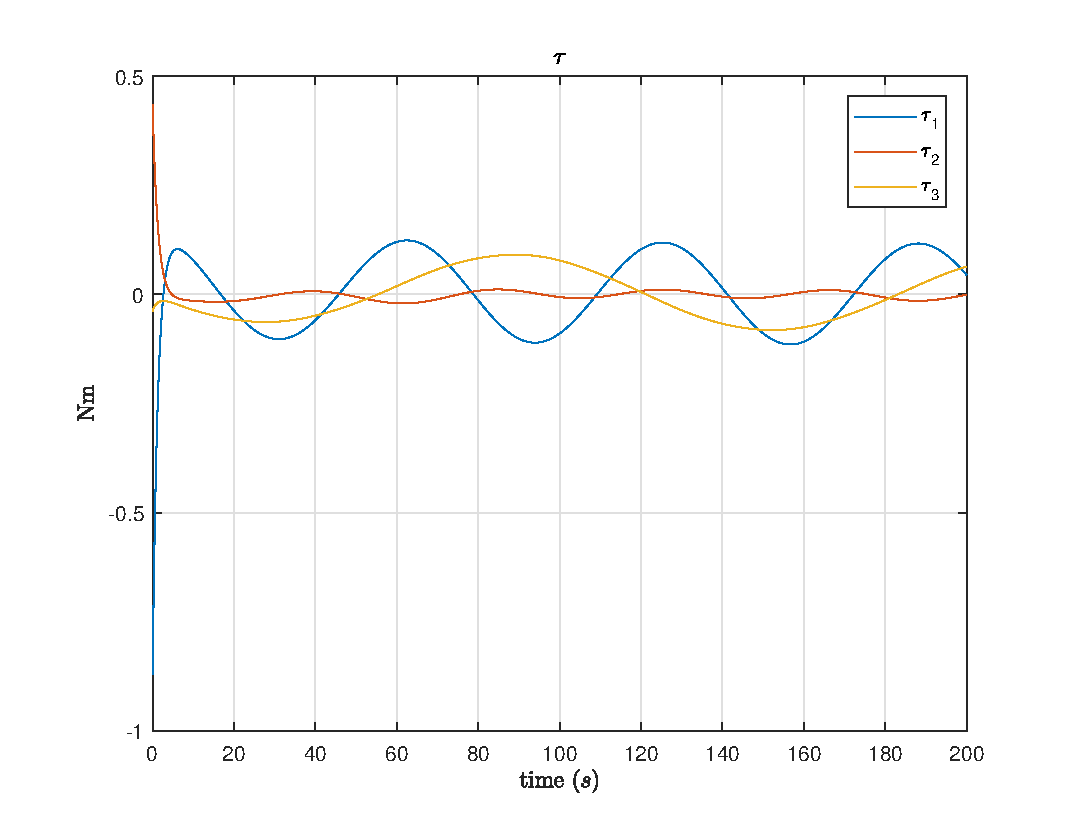
\includegraphics[scale=0.95]{tau2.eps}
    \caption{Simulated control input $\tau$}
    \label{fig:tau2}
\end{figure}
